\documentclass[a4paper,10pt]{article}

% Encoding.
\usepackage{geometry}
\usepackage[T2A]{fontenc}
\usepackage[utf8]{inputenc}
\usepackage[english,russian]{babel}

% No line breaks.
\usepackage[none]{hyphenat}

% Links are clickable.
\usepackage{hyperref}

% Image insertion.
\usepackage{svg}

% Math functions.
\usepackage{amsmath}

% Code insertion.
\usepackage[outputdir=build]{minted}

\title{\textbf{Техническое задание \\ на разработку модуля \\ SUPERLIB} \\
       \large Версия 1.0}
\author{ Смирнов Александр }
\date{\today}

\renewcommand{\contentsname}{Whatever}

\begin{document}


    \maketitle


    \tableofcontents
    \newpage
     
    \section{Введение}

 
        Данный документ является техническим заданием на разработку модуля \textbf{SUPERLIB} для компании \textbf{NG}.  

         
        Новый модуль будет независимой составной частью системы автоматизации.

    \section{Общие требования}


        Приложение \textbf{SUPERLIB} -- система, ориентированная на учёт выдачи и возврата книг в библиотеке, регистрацию запросов на книги и резервирование книг. 

        Сотрудник библиотеки регистрирует выданные посетителю и возвращенные им книги. Данные о выданных книгах сохраняются в истории выдач. Если нужная посетителю книга в данный момент находится на руках, сотрудник библиотеки регистрирует запрос на нее и ставит его в очередь ожидания. Если посетитель хочет зарезервировать за собой книгу на определенный период времени, сотрудник библиотеки проверяет, нет ли заказов на резервирование этой книги на этот период и, если их нет, резервирует книгу для данного посетителя на данный период.  

        В приложении предусмотрена следующуя возможность: самым активным посетителям присылается по почте оповещение о новых поступлениях книг наиболее предпочитаемого ими типа.


    \newpage

    \section{Подробное описание модуля}

        \subsection{Технические требования}

         
            Приложение \textbf{SUPERLIB} должно функционировать как web-приложение и работать под следующими web-браузерами: 
             
            \begin{itemize}
                \item Google Chome
                \item IE 
                \item FireFox 
                \item Safary 
                \item Opera 
            \end{itemize}
            
         
        \subsection{Категории пользователей }

         
            Приложение \textbf{SUPERLIB} будет ориентировано на следующие категории пользователей: 

            \begin{itemize}
                \item Сотрудник библиотеки
                \item Суперпользователь
                \item Клиент (посетитель библиотеки)
            \end{itemize}

        \subsection{Состояние книги}

            При выдаче книги прослеживаются следующие состояния:

            \begin{itemize}
                \item В библиотеке
                \item Выдана посетителю
                \item В списке ожидания
            \end{itemize}

        \newpage

        \subsection{Функциональность приложения}

         
            \subsubsection{Сотрудник библиотеки}

                \begin{itemize}
                    \item Регистрация нового посетителя
                        \begin{itemize}
                            \item ФИО
                            \item паспортные данные
                            \item электронный адрес
                            \item телефон
                        \end{itemize}
                    \item Редактирование данных посетителя
                    \item Добавление новой книги
                        \begin{itemize}
                            \item название
                            \item автор
                            \item издатель
                            \item год выпуска
                        \end{itemize}
                    \item Редактирование данных книги
                    \item Добавление книги в таблицу выданных книг
                        \begin{itemize}
                            \item посетитель
                            \item книга
                            \item дата получения 
                            \item дата возврата
                        \end{itemize}
                    \item Редактирование даты возврата выданной книги
                    \item Добавление книги в таблицу очереди
                        \begin{itemize}
                            \item посетитель
                            \item книга
                            \item дата получения 
                            \item дата возврата
                        \end{itemize}
                    \item Редактирование и удаление записей в таблице очередей
                    \item Получение отчётов по выданным книгам
                \end{itemize}


            \newpage


            \subsubsection{Суперпользователь}

                \begin{itemize}
                    \item Регистрация нового сотрудника библиотеки
                        \begin{itemize}
                            \item ФИО
                            \item паспортные данные
                            \item электронный адрес
                            \item телефон
                        \end{itemize}
                    \item Редактирование данных сотрудника библиотеки
                    \item Изменение / редактирование любых данных
                \end{itemize}


            \subsubsection{Клиент (посетитель библиотеки)}

                \begin{itemize}
                    \item Напоминание о возврате книги
                    \item Оповещение о новых поступлениях опираясь на историю чтения
                \end{itemize}


    \newpage


    \section{Спецификация}

        \subsection{База данных}

            Для учёта выданных книг нужно будет созданить несколько таблиц в базе данных \textbf{LIBRARY}:

            \begin{figure}[h]
                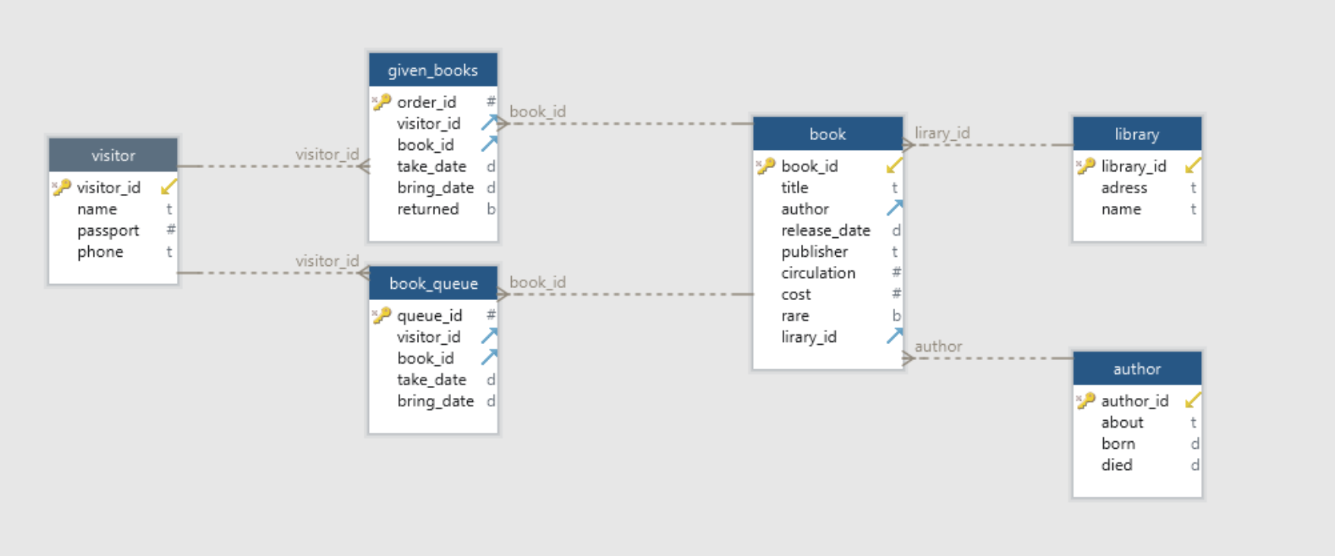
\includegraphics[width=1.0\textwidth]{./images/db.png}
                \centering
            \end{figure}

            Пояснение к объектам БД:

            \begin{table}[h]
                \centering
                \begin{tabular}{|l|l|}
                    \hline
                    \multicolumn{1}{|c|}{\textbf{Таблица}} & \multicolumn{1}{c|}{\textbf{Назначение}} \\ \hline
                    visitor                                & Данных о посетителях                     \\ \hline
                    library                                & Данные о библиотеках                     \\ \hline
                    book                                   & Данные о книгах                          \\ \hline
                    author                                 & Данные об авторах                        \\ \hline
                    given\_books                           & Данные о выданных книгах                 \\ \hline
                    book\_queue                            & Очередь на книги                         \\ \hline
                \end{tabular}
            \end{table}

    \newpage

        \subsection{Web-приложение}

             
            В приложении должна быть реализована вся функциональность, описанная выше.

            \subsubsection{Интерфейсы}


                \begin{itemize}
                    \item Добавить пользователя
                    \item Добавить книгу
                    \item Добавить книгу в таблицу выданных книг
                    \item Добавить книгу в очередь
                \end{itemize}

            \subsubsection{Отчёты}


                \begin{itemize}
                    \item Список выданных книг
                    \item Список книг в библиотеке
                    \item Список пользователей, которые должны вернуть книги
                \end{itemize}


\end{document}
